%%%%%%%%%%%%%%%%%%%%%%%%%%%%% ANEXO %%%%%%%%%%%%%%%%%%%%%%%%%%%%%

%\section*{\centering{A – ANEXOS Y APÉNDICES }} % Añadir código
%\addcontentsline{toc}{section}{A - ANEXOS Y APÉNDICES}

% Los anexos y apéndices son materiales adicionales, utilizados para complementar el texto, añadidos al final del trabajo, con la finalidad de aclaración o de comprobación. Son elaborados por el autor y pretenden complementar una argumentación y sirven de fundamentación teórica, comprobación e ilustración (por ejemplo, mapas, leyes, códigos)

%\chapter*{Apendice A - }
%\label{ch:Apendice}

%\section*{\huge Apéndice A} 
%\section*{Fuentes de información para la descarga de MDT}
%\addcontentsline{toc}{chapter}{Apéndice A: Fuentes de información para descarga de MDT}

%\begin{itemize}
%	\item \item \url{https://www.cursosteledeteccion.com/fuentes-gratuitas-para-descargar-dem-modelo-de-elevacion-digital/}
%	\item \url{http://www.gisandbeers.com/descarga-de-dem-mundiales-mde/}
%	\item \url{https://gisgeography.com/free-global-dem-data-sources/}
%	\item \url{http://www.gpsvisualizer.com/elevation}
%	\item \url{https://mappinggis.com/2017/12/programas-gratuitos-para-trabajar-con-imagenes-de-satelite/}
%\end{itemize}

\newpage

\section*{\huge Apéndice C} 
\section*{Instalación de GraphDB}
\label{ch:ApendiceC}
\addcontentsline{toc}{chapter}{Apéndice C: Instalación de GraphD}

%\chapter*{Apéndice B: Instalación de GraphD}
%\subsection{Tipos de Web} % Evolución de la Web

\textit{\textbf{Nota}: La instalación y uso de GraphDB se ha hecho en macOS 10.14}\\

\textbf{GraphDB} es una base de datos de grafos semánticos, que cumple con los estándares W3C. Proporciona la infraestructura central para soluciones donde la agilidad de modelado, la integración de datos, la exploración de relaciones y la publicación y consumo de datos son importantes. Además, su uso nos ha permitido solventar los problemas ocasionados con Protegé para la realización de las consultas con información geográfica georreferenciada. Es por eso que es indispensable conocer las requisitos que necesita y los pasos para su correcta instalación. Para instalar GraphDB debemos acceder a la página \url{http://graphdb.ontotext.com} y descargarnos la última versión de \textit{GraphDB Free}, tal como lo vemos en la figura \ref{fig:1}. Hemos descargado la versión gratuita de este software. Previamente a la descarga de este software es necesario cumplimentar un breve formulario (figura \ref{fig:3}). Además, como GraphDB es una aplicación Java, requiere de Java 8 (\url{https://java.com/en/download/help/download_options.xml}).

\begin{figure}[H]
	\centering
	\begin{subfigure}[h]{0.72\textwidth} 
		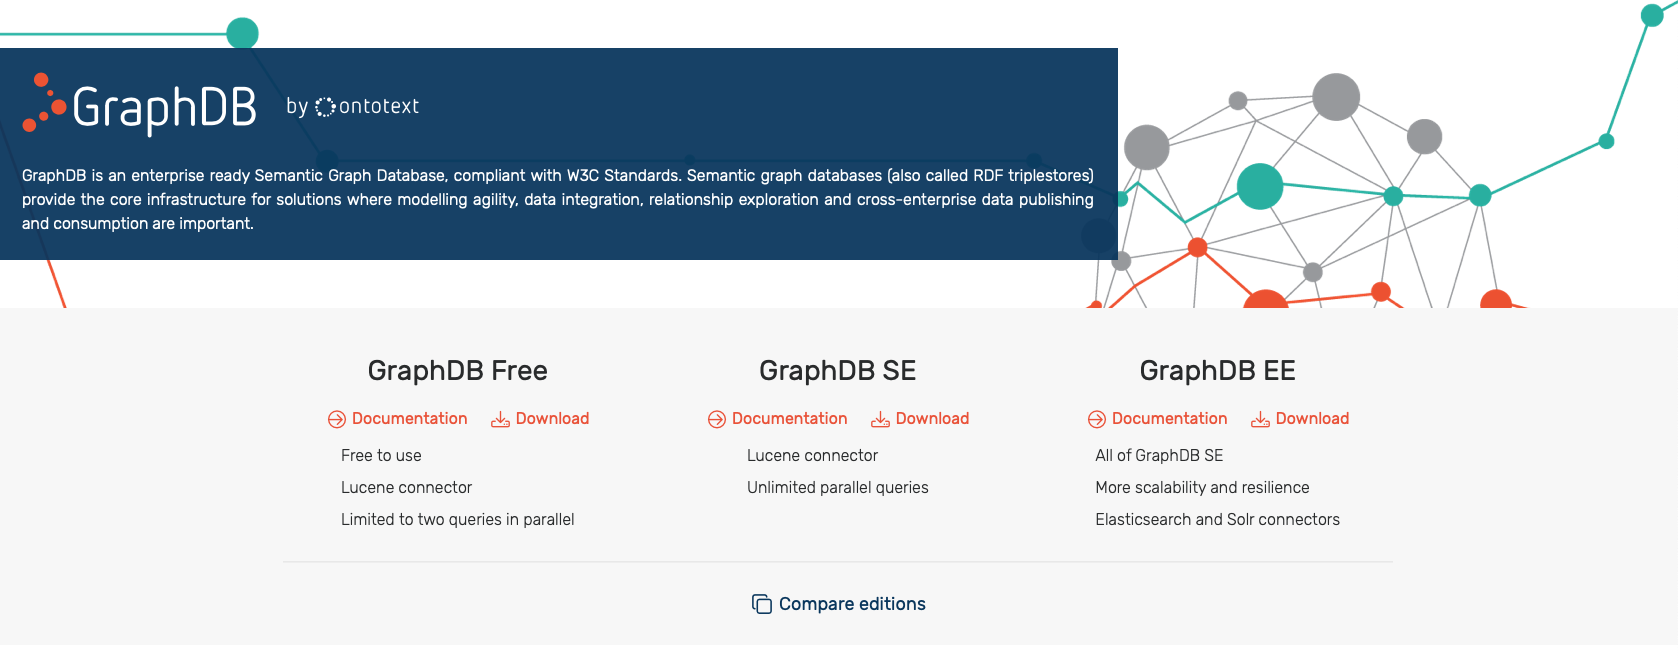
\includegraphics[width=\textwidth]{imagenes/apendices/1}
		\caption{}
	\end{subfigure}       
	\begin{subfigure}[h]{0.72\textwidth} 
		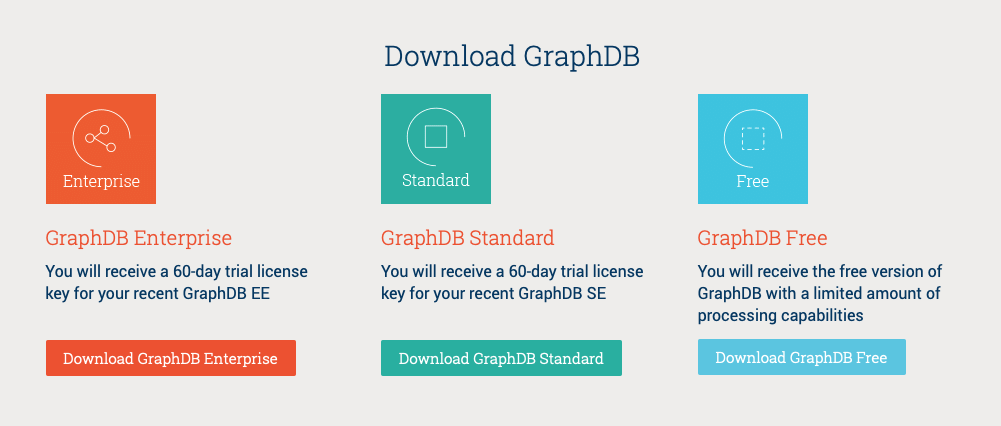
\includegraphics[width=\textwidth]{imagenes/apendices/2}
		\caption{}
	\end{subfigure}
	\caption{Página para la descarga de GraphDB Free}
	\label{fig:1}
\end{figure}

\begin{figure}[H]
	\centering
	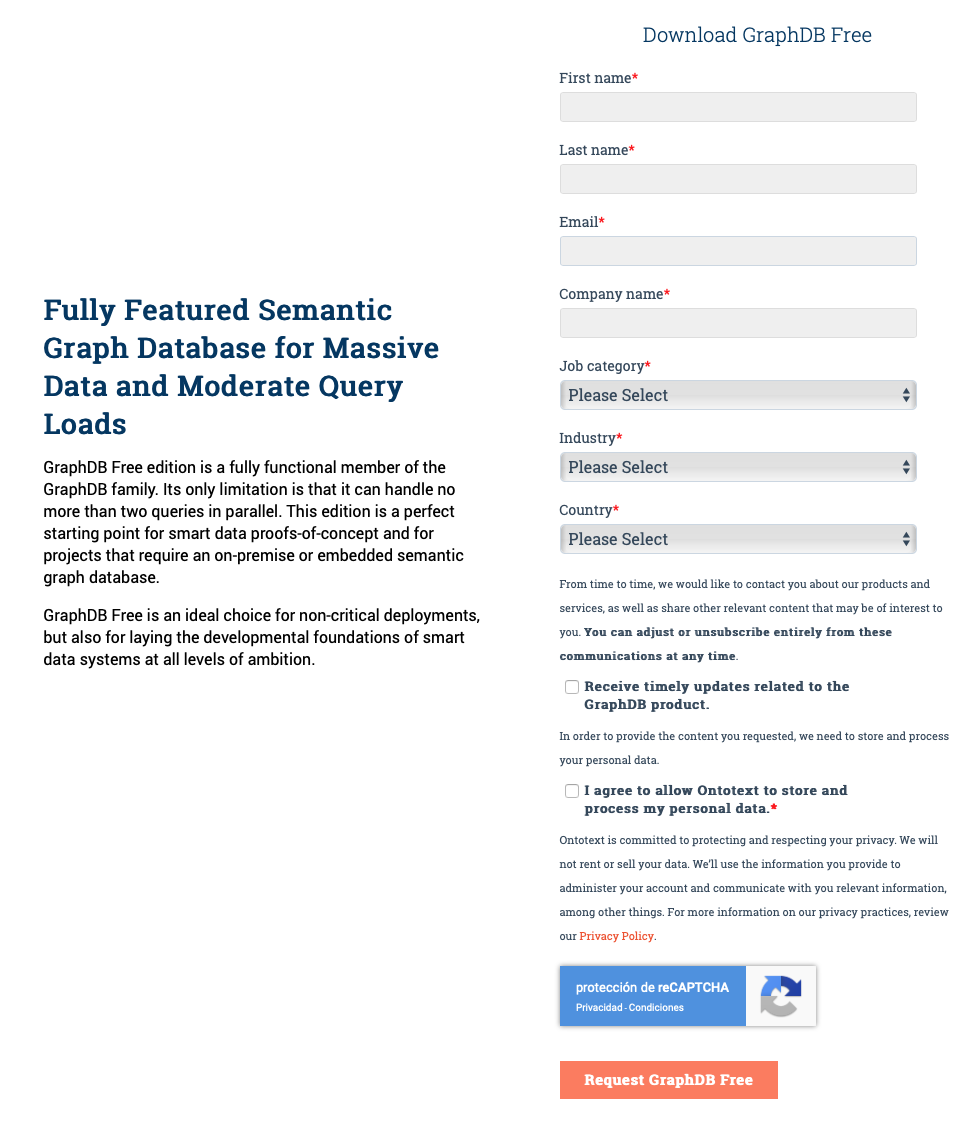
\includegraphics[width=0.73\linewidth]{imagenes/apendices/3}
	\caption{Formulario para iniciar la descarga de GraphDB Free}
	\label{fig:3}
\end{figure}

Una vez terminada la descargada (nos hemos descargado la última versión), tendremos un zip descargado con el nombre de \textit{graphdb-free-8.10.1}. Al descomprimir la carpeta, y teniendo Java instalado, es posible iniciar GraphDB, para ello es necesario ejecutar el script \textit{graphdb} en el directorio \texttt{bin} (figura \ref{fig:4}). Para acceder al \textit{Workbench}, abrimos en el navegador la siguiente direccción \url{http://localhost:7200} (figura \ref{fig:5}).\\

\begin{lstlisting}
# Version de Java
$ java -version
java version "1.8.0_212"
Java(TM) SE Runtime Environment (build 1.8.0_212-b10)
Java HotSpot(TM) 64-Bit Server VM (build 25.212-b10)
\end{lstlisting}

\begin{lstlisting}
# Dirigirse al directorio bin
$ cd graphdb-free-8.10.1/bin/

# Ejecutar el script graphdb 
$ ./graphdb
\end{lstlisting}

\begin{figure}[H]
	\centering
	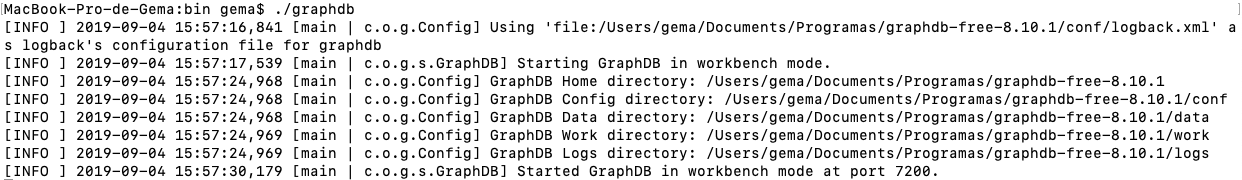
\includegraphics[width=1\linewidth]{imagenes/apendices/4}
	\caption{Iniciando GrapbDB en el terminal}
	\label{fig:4}
\end{figure}


\begin{figure}[H]
	\centering
	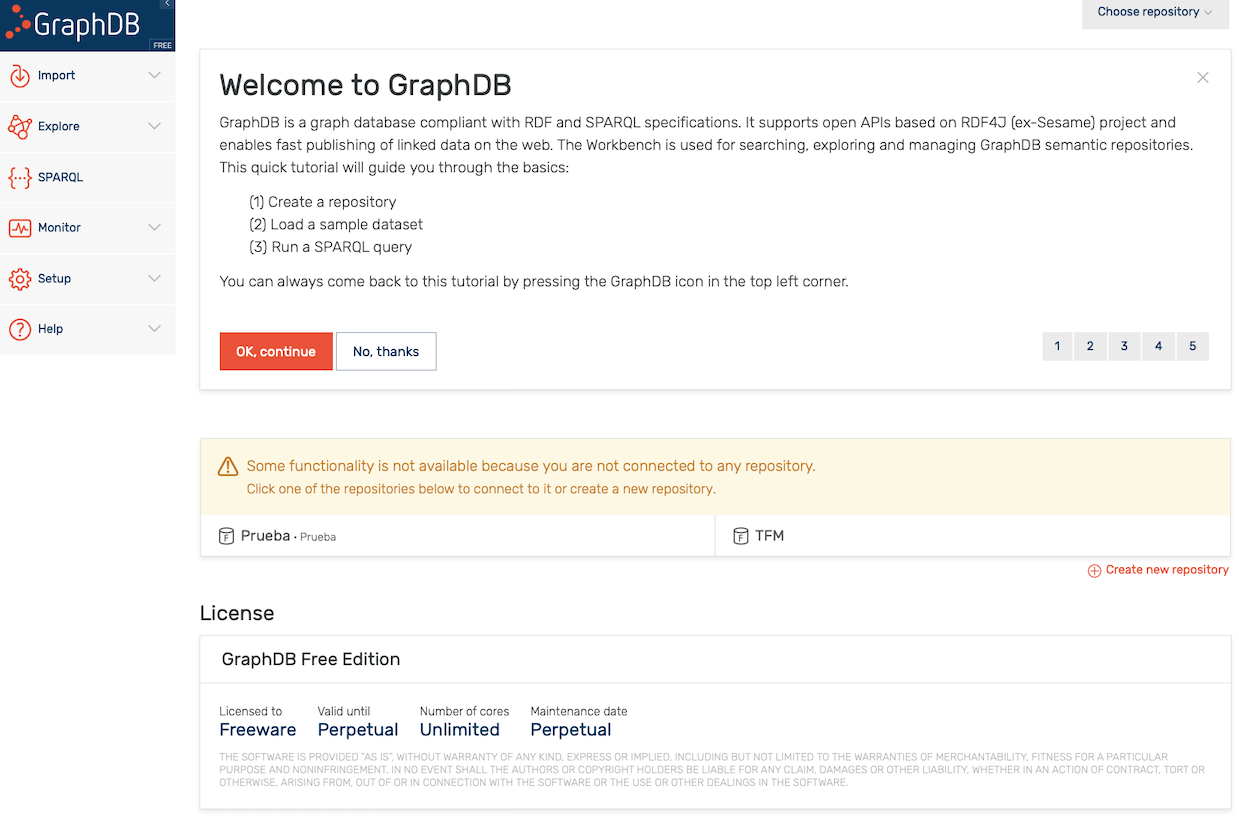
\includegraphics[width=1\linewidth]{imagenes/apendices/5}
	\caption{Página de inicio de GraphDB en \url{http://localhost:7200}}
	\label{fig:5}
\end{figure}

Por último y no menos importante, es necesario crear un repositorio (\texttt{Setup>Repositories}) y conectarse a él, para poder hacer todas las consultas que hemos visto anteriormente.

\begin{figure}[H]
	\centering
	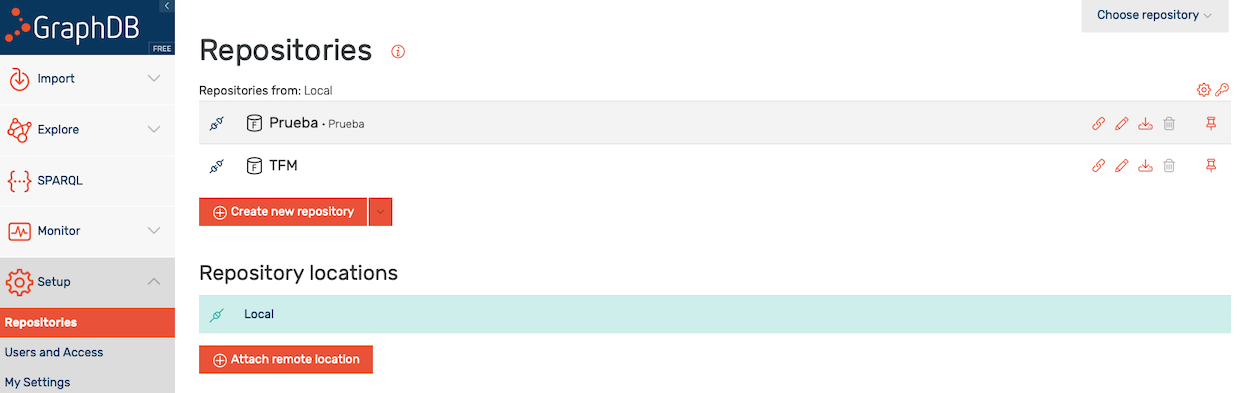
\includegraphics[width=1\linewidth]{imagenes/apendices/repo}
	\caption{Página para crear un nuevo repositorio en GraphDB}
	\label{fig:repo}
\end{figure}

\textit{Si se quiere saber más información acerca de GraphDB, es posible acceder a su documentación en la dirección \url{http://graphdb.ontotext.com/documentation/free/}, la cual contiene información muy útil y muy bien explicada.}



